% TikZ 复刻。原图：assets/mirror-placement.png
% 回退：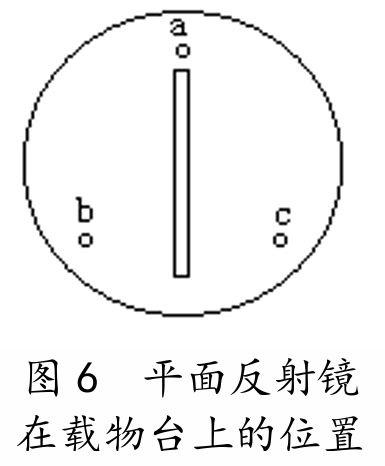
\includegraphics[width=0.32\linewidth]{assets/mirror-placement.png}
\begin{tikzpicture}[font=\small]
  \def\R{2.05}
  \draw[thick] (0,0) circle (\R);
  \foreach \ang in {90,210,330} {
    \draw[thin] (0,0) -- (\ang:\R);
  }
  \filldraw[fill=white, thick] (90:\R) circle (0.16);
  \filldraw[fill=white, thick] (210:\R) circle (0.16);
  \filldraw[fill=white, thick] (330:\R) circle (0.16);
  \node[above=5pt] at (90:\R) {$a$};
  \node[below left] at (210:\R) {$b$};
  \node[below right] at (330:\R) {$c$};
  \filldraw[fill=gray!20, thick] (-0.11,-1.20) rectangle (0.11,1.15);
  \node[right] at (1.15,-0.15) {反射镜};
  \draw[thin] (0.11,0.05) -- (1.05,-0.12);
\end{tikzpicture}
